\chapter{Basic primitives}
{ }\hfill\textbf{Level:} newbie\\ \\
\noindent
To move the turtle on the drawing area, we use predefined commands called ``primitives''. In this chapter, we're going to discover the basic primitives allowing us to pilot the turtle on the drawing area.
\section{New primitives}
\begin{itemize}
\item \texttt{forward number }\hspace {4cm } \textcolor{red}{ \texttt{fd 50}}\\
 Moves the turtle forward number of steps in the direction it is currently facing.
\item \texttt{back number}\hspace {4cm } \textcolor{red}{ \texttt{bk 100}}\\
Moves the turtle backwards number of steps in the direction it is currently facing.
\item \texttt{right number}\hspace {4cm } \textcolor{red}{\texttt{rt 90}}\\
 Turns the turtle towards the right in relation to the direction it is currently facing.
\item \texttt{left number}\hspace {4cm } \textcolor{red}{ \texttt{lt 45}}\\
 Turns the turtle  towards the left in relation to the direction it is currently facing.
\item \texttt{clearscreen}\hspace {4cm } \textcolor{red}{ \texttt{cs}}\\
Erases the drawing area.
\item \texttt{showturtle}\hspace {4cm } \textcolor{red}{ \texttt{st}}\\
The turtle is visible on screen.
\item \texttt{hideturtle}\hspace {4cm } \textcolor{red}{ \texttt{ht}}\\
The turtle is invisible (drawing is faster).
\item \texttt{penup}\hspace {4cm } \textcolor{red}{ \texttt{pu}}\\
The turtle won't draw a line when it moves.
\item \texttt{pendown}\hspace {4cm } \textcolor{red}{ \texttt{pd}}\\
The turtle will draw a line when it moves.
\item \texttt{repeat integer list}\hspace {4cm } \textcolor{red}{ \texttt{repeat 5[fd 50 rt 45]}}\\
Repeat instructions contained in the list.
\end{itemize}
\section{Drawing a regular polygon}
\noindent In this part, we'll learn to draw a square, equilateral triangle, and a regular polygon in general....
\subsection{Square}
\begin{center}
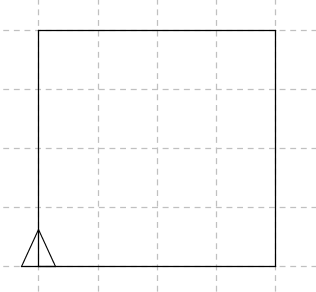
\includegraphics{pics/bases-carre.png}
\end{center}
\noindent To draw this square, we're going to write:
\begin{verbatim}
fd 200 rt 90 fd 200 rt 90 fd 200 rt 90 fd 200 rt 90
\end{verbatim}
We can see that we repeat $4$ times the same instructions. Therefore, a better syntax:
\begin{verbatim}
repeat 4[fd 200 rt 90]
\end{verbatim}
\subsection{Equilatéral triangle}
\begin{center}
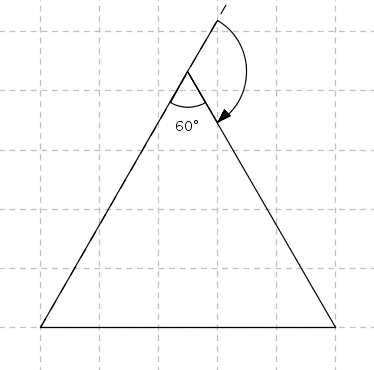
\includegraphics{pics/bases-triangle.png}
\end{center}
\noindent Here, we'll learn how to draw this equilatéral triangle (all three sides have 150 steps lengths).\\ \\
The command will have this form: 
\begin{verbatim}
repeat 3[fd 150 rt ....]
\end{verbatim}
We must determinate the angle. In an equilateral triangle, all three internal angles are equal to each other and so are each 60 degrees. The turtles turns outside the triangle. Hence, the value for this angle is 180-60=120 degrees. The valid command is:
\begin{verbatim}
repeat 3[fd 150 rt 120]
\end{verbatim}
\subsection{Hexagon}
\begin{center}
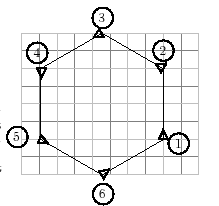
\includegraphics{pics/bases-hexagone.png}
\end{center}
\noindent \begin{verbatim}
repeat 6[fd 80 rt ....]
\end{verbatim}
When the turtle has finished its moves, it has made one tour from its initial position to its final position. This is done using 6 steps. Therefore, each angle value is equal to  $\dfrac{360}{6}=60\textrm{\degre}$. \\ \\
The valid command is: \texttt{repeat 6[fd 80 rt 60]}

\subsection{Drawing a regual polygon in general}
\noindent In fact, the reasoning makes us think that to draw a polygon with $n$ sides, the turtle will have to turn from an angle whose value is 360 divided by $n$. For example:
\begin{itemize}
\item To draw a regular pentagon with side length 100:
\begin{verbatim}
repeat 5[fd 100 rt 72]    (360:5=72)
\end{verbatim}
\item To draw a nine sided polygon with side length 20:
\begin{verbatim}
repeat 9[fd 20 rt 40]    (360:9=40)
\end{verbatim}
\item To draw hum... a regular 360-gon with side length 2:
\begin{verbatim}
repeat 360[fd 2 rt 1]  
\end{verbatim}
This form is really near a circle!
\item To draw an heptagon with  side length 120:
\begin{verbatim}
repeat 7[fd 120 rt 360/7]
\end{verbatim}
\end{itemize}

\section{Saving a procedure}
\noindent Because we do not wish to rewrite each time the same instructions to draw a square, a triangle... it's better to save these instructions into a ``procedure''. To define a procedure, open the editor. A procedure starts with the keyword \texttt{to} and finishes with the keyword \texttt{end}. To define a square procedure:
\begin{verbatim}
to square
repeat 4[fd 100 rt 90]
end
\end{verbatim}
then we close the editor by clicking on the turtle button. It will save the editor contents. Now, when we write \texttt{square} in the command line, a square appears on screen!

\section{Exercice ...}
\noindent Each square is 10 steps wide. Try to draw this image defining eight procedures:
\begin{itemize}
\item A procedure called \texttt{square} that draws the main square of the house.
\item A procedure called \texttt{triangle} that draws the roof as an equilateral triangle.
\item A procedure called \texttt{door} that draws the rectangular door.
\item A procedure called \texttt{chimney} that draws the chimney.
\item A procedure called \texttt{move1} that allows the turtle to move from point A to point B.
\item A procedure called \texttt{move2} that allows the turtle to move from point B to point C.
\item A procedure called \texttt{move3} that allows the turtle to move from point C to point D. (Warning: you'll have to pen up!)
\item A general procedure called  \texttt{house} that draws the whole house using all previous procedures.
\end{itemize}
\label{maison}
\begin{center}
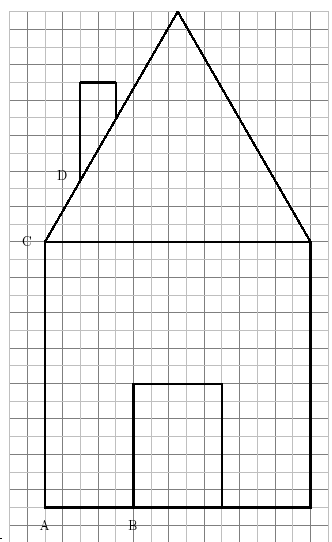
\includegraphics[scale=0.6]{pics/bases-maison.png}
\end{center}